\documentclass{article}
\usepackage{amsmath,amscd,amsbsy,amssymb,latexsym,url,bm,amsthm}
\usepackage{epsfig,graphicx,subfigure}
\usepackage{enumitem,balance}
\usepackage{wrapfig}
\usepackage{mathrsfs, euscript}
\usepackage[usenames]{xcolor}
\usepackage{hyperref}
\usepackage[vlined,ruled,commentsnumbered,linesnumbered]{algorithm2e}

\newtheorem{theorem}{Theorem}[section]
\newtheorem{lemma}[theorem]{Lemma}
\newtheorem{proposition}[theorem]{Proposition}
\newtheorem{corollary}[theorem]{Corollary}
\newtheorem{exercise}{Exercise}[section]
\newtheorem*{solution}{Solution}
\theoremstyle{definition}
\hypersetup{hidelinks}


\numberwithin{equation}{section}
\numberwithin{figure}{section}

\renewcommand{\thefootnote}{\fnsymbol{footnote}}

\newcommand{\postscript}[2]
 {\setlength{\epsfxsize}{#2\hsize}
  \centerline{\epsfbox{#1}}}

\renewcommand{\baselinestretch}{1.0}


\makeatletter \renewenvironment{proof}[1][Proof] {\par\pushQED{\qed}\normalfont\topsep6\p@\@plus6\p@\relax\trivlist\item[\hskip\labelsep\bfseries#1\@addpunct{.}]\ignorespaces}{\popQED\endtrivlist\@endpefalse} \makeatother
\makeatletter
\renewenvironment{solution}[1][Solution] {\par\pushQED{\qed}\normalfont\topsep6\p@\@plus6\p@\relax\trivlist\item[\hskip\labelsep\bfseries#1\@addpunct{.}]\ignorespaces}{\popQED\endtrivlist\@endpefalse} \makeatother



\begin{document}
\noindent

%========================================================================
\noindent\framebox[\linewidth]{\shortstack[c]{
\Large{\textbf{Homework 1}}\vspace{1mm}\\
CS420-Machine learning, Shikui Tu, Spring 2018}}
\begin{center}

\footnotesize{\color{blue}$*$ Name:Zhiwen Qiang  \quad Student ID:515030910367 \quad Email: qlightman@163.com}
\end{center}

\section{k--mean vs GMM}

Give a variant of k--mean algorithm somewhat between the original k--mean and Expectation-Maximization (EM) for Gaussian Mixture Models (GMM). Please specify the computational details of the formulas. Pseudo-codes of the algorithm would be great.\\
Discuss the advantages or limitations of your algorithm.
\subsection{Computational Details}
FCM is a kind of fuzzy clustering algorithm, which allows data to belong to two or more clusters. It is based on minimization $J_m$, where $J_m$ refer to:
\begin{equation}
J_m=\sum^N_{i=1}\sum_{j=1}^{C}u_{ij}^m||x_i-c_j||^2, \qquad 1\leq m \le \infty
\label{equ1}
\end{equation}
$m$ is a real number greater than 1, $u_{ij}$ is the degree of $x_i$ in cluster $j$, $x_i$ is the $i$th of d-dimensional data, $c_j$ is the d-dimension center of the cluster.

The fuzzy operation is carried out through an iterative optimization of the objective function shown in equation \ref{equ1}, $u_{ij}$ and $c_j$ is defined in equation 1.2, 1.3.
\begin{equation}
u_{ij}=\frac{1}{\sum^C_{k=1}(\frac{||x_i-c_j||}{||x_i-c_k||})^{\frac{2}{m-1}}}
\label{euq2}
\end{equation}

\begin{equation}
c_j=\frac{\sum_{i=1}^Nu_{ij}^mx_i}{\sum_{i=1}^Nu_{ij}^m}
\label{euq3}
\end{equation}
The iteration won't stop until $max(|u_{ij}^{k+1}-u_{ij}^{(k)}|)<\varepsilon$, where $\varepsilon$ is a termination criterion range form 0 to 1.

\subsection{Pseudo-codes}
\begin{algorithm}[H]
		\BlankLine
		\SetKwInOut{Input}{input}
		\SetKwInOut{Output}{output}
		\caption{FCM algorithm}\label{FCM}
		\Input{A batch of data points.}
		\Output{Dataset being divided into several groups.}
		\BlankLine
        Initialize $U=[u_{ij}]$ matirx, $U^{0}$ \\
        
        
		\While{$||U^{k+1}-U^{k}||>=\varepsilon$}{
		     At k-step: calculate the centers vectors $C^{k}=[c_j]$ with $U^{k}$\\
		     Update $U^{k}$,$U^{k+1}$
		}
	\end{algorithm}

\subsection{Advantages}
\begin{itemize}
\item In overlapped data set, the result is comparatively better than k-means algorithm.
\item Unlike k-means algorithm, the data point in FCM may belong to one or more clusters, which suits well in a lot more situations. 
\end{itemize}
\subsection{Limitations}
\begin{itemize}
\item The number of iterations are usually large, thus requires more time to compute than k-means algorithm. 
\item This algorithm is sensitive to isolated points.
\end{itemize}

\section{k--mean vs CL}
Compare the k--mean algorithm with competitive learning (CL) algorithm. Could you apply the
idea of Rival Penalized Competitive Learning (RPCL) to k-mean so that the number of clusters
is automatically determined? If so, give the details of your algorithm and then implement it on a
three-cluster dataset generated by yourself. If not, state the reasons.

\subsection{Comparision}
\begin{itemize}
\item Competitive learning algorithm is an adaptive way of learning. To be specific, in clustering problems, competitive learning algorithm usually view problem in an adaptive way, that is: data points come one by one. While in k-means algorithm, it usually deals with a batch of data points.
\item Competitive learning algorithm is a form of unsupervised learning in artificial neural networks, which is a more general type of algorithms, it includes RPCL, FSCL, etc. While k-means algorithm is more specific and only deals with the clustering problems.
\item K-means algorithm use a 'winner takes all' strategy, which may perform badly when starting with 'bad initializations'. On the other hand, FSCL algorithm solve the problems by penalizing the frequent winners. Also, k-means cannot determine the number of clusters, while RPCL can automatically determine the $k$ value by penalizing the 'rivel'. So in a word, CL algorithm is more general and can deal with many situations where the k-means cannot handle.

\end{itemize}

\subsection{Solution}
I think it is possible to apply the RPCL to k-means so that the number of clusters is automatically determined. The way to locate the extra center is by examing the distances between each centers. I assume that the extra center is cutting apart some of the points in other center, so after each time the center of each cluster is relocated, we need to select the two centers where their distance is the shortest.
Then kick the center where its group is smaller than the other point away to some ratio.
The pseudo-code of this algorithm is defined below:\\\\
\begin{algorithm}[H]
		\BlankLine
		\SetKwInOut{Input}{input}
		\SetKwInOut{Output}{output}
		\caption{RPCL-k-means algorithm}\label{RPCL}
		\Input{An three-cluster dataset.}
		\Output{Dataset being divided into several groups.}
		\BlankLine
        Initialize $m_i$, $i=1,\dots,k$ 
		\While{$m_i$ don't converge}{
		     \For {all $x$ in $X$}{
		          if($||x-m_i=min_j||x-m_j||$)$b_i\leftarrow 1$\\
		          else $b_i\leftarrow0$
		     }
		     \For{all $m_i$, $i=1,\dots,k$}{
		        $m_i \leftarrow \sum b_ix/\sum b_i$
		     }
		     \For{all $m_i$, $i=1,\dots,k$}{
		     	select the two points where their distance is the shortest.\\
		     	kick the point where its group is smaller than the other point away to some ratio.
		     	}
		}
	\end{algorithm}

\subsection{Results}
Figure \ref{data} is the three-cluster dataset I generated, figure \ref{normal} is the results obtained from normal k-means algorithm. The given $k$ value is 4 and it is obvious that the result isn't good. In figure \ref{6times} we present the results obtaind form the RPCL-k-means algorithm, we can see that point resprenting the extra center is being 'kicking' away, which proves the correctness of my algorithm. (Pictures of other interations can be found in the 'picture' folder)
\begin{figure}[htbp]
	\centering
	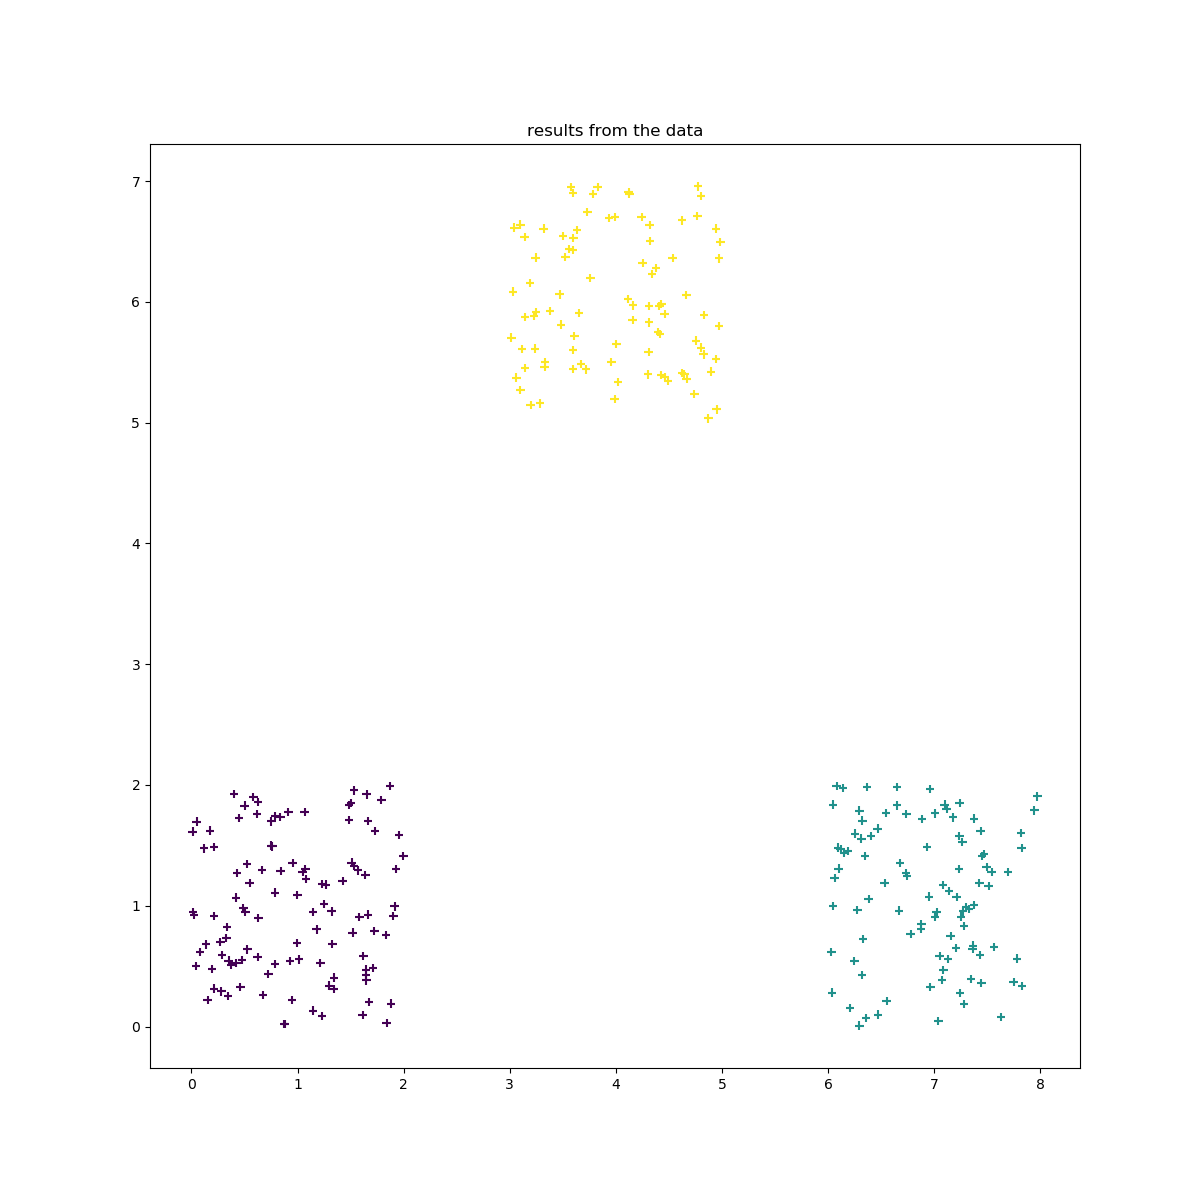
\includegraphics[width=10cm]{problem2/data.png}
\caption{The three-cluster dataset I generated.}
\label{data}
\end{figure}

\begin{figure}[htbp]
	\centering
	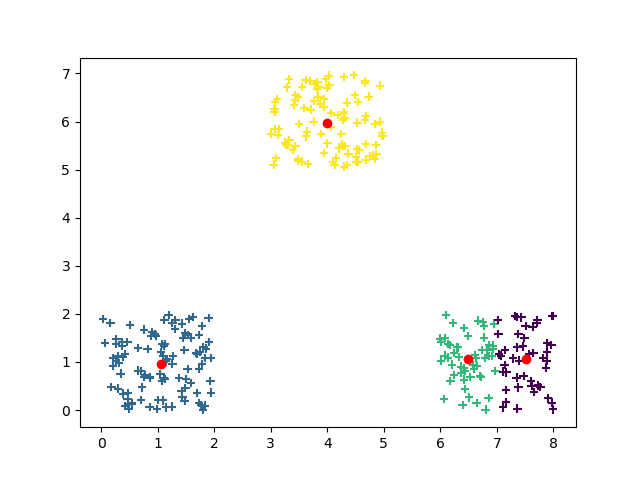
\includegraphics[width=10cm]{problem2/normal_k_means.png}
\caption{Results obtained from normal k-means algorithm.}
\label{normal}
\end{figure}


\begin{figure}[htbp]
	\centering
	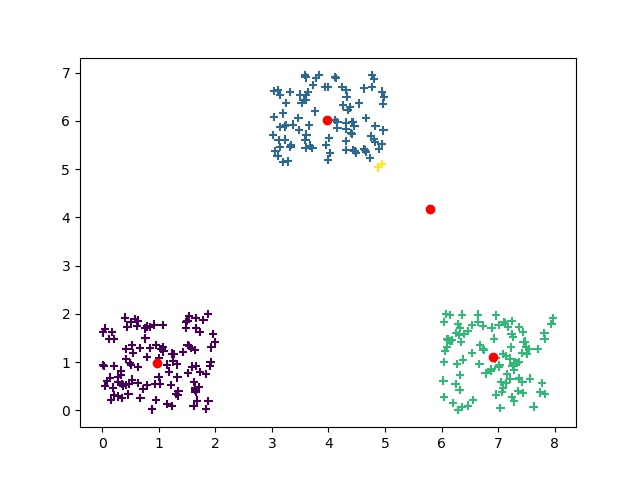
\includegraphics[width=10cm]{problem2/iterations/6interations.jpg}
\caption{Results obtained from RPCL-k-means algorithm in 6 interations}
\label{6times}
\end{figure}

\section{model selection of GMM}
Write a report on experimental comparisons on model selection performance between BIC,AIC and
VBEM. Specifically, you need to randomly generate datasets based on GMM, by varying some factors, e.g.,
sample sizes, dimensionality, number of clusters, and so on.
\subsection{BIC}
Using the sklearn mixture module, we implement a example in Figure \ref{BIC}, first we
 randomly generate datasets based on GMM, in this case, the dataset consists of 3 components, then run the algorithm on the dataset for $k=1\dots 6$, the result is shown in the bar chart, the rectangle with $*$ above it is the best match. It is the model with 3 components and full covariance, which is the true generative model.
\begin{figure}[htbp]
	\centering
	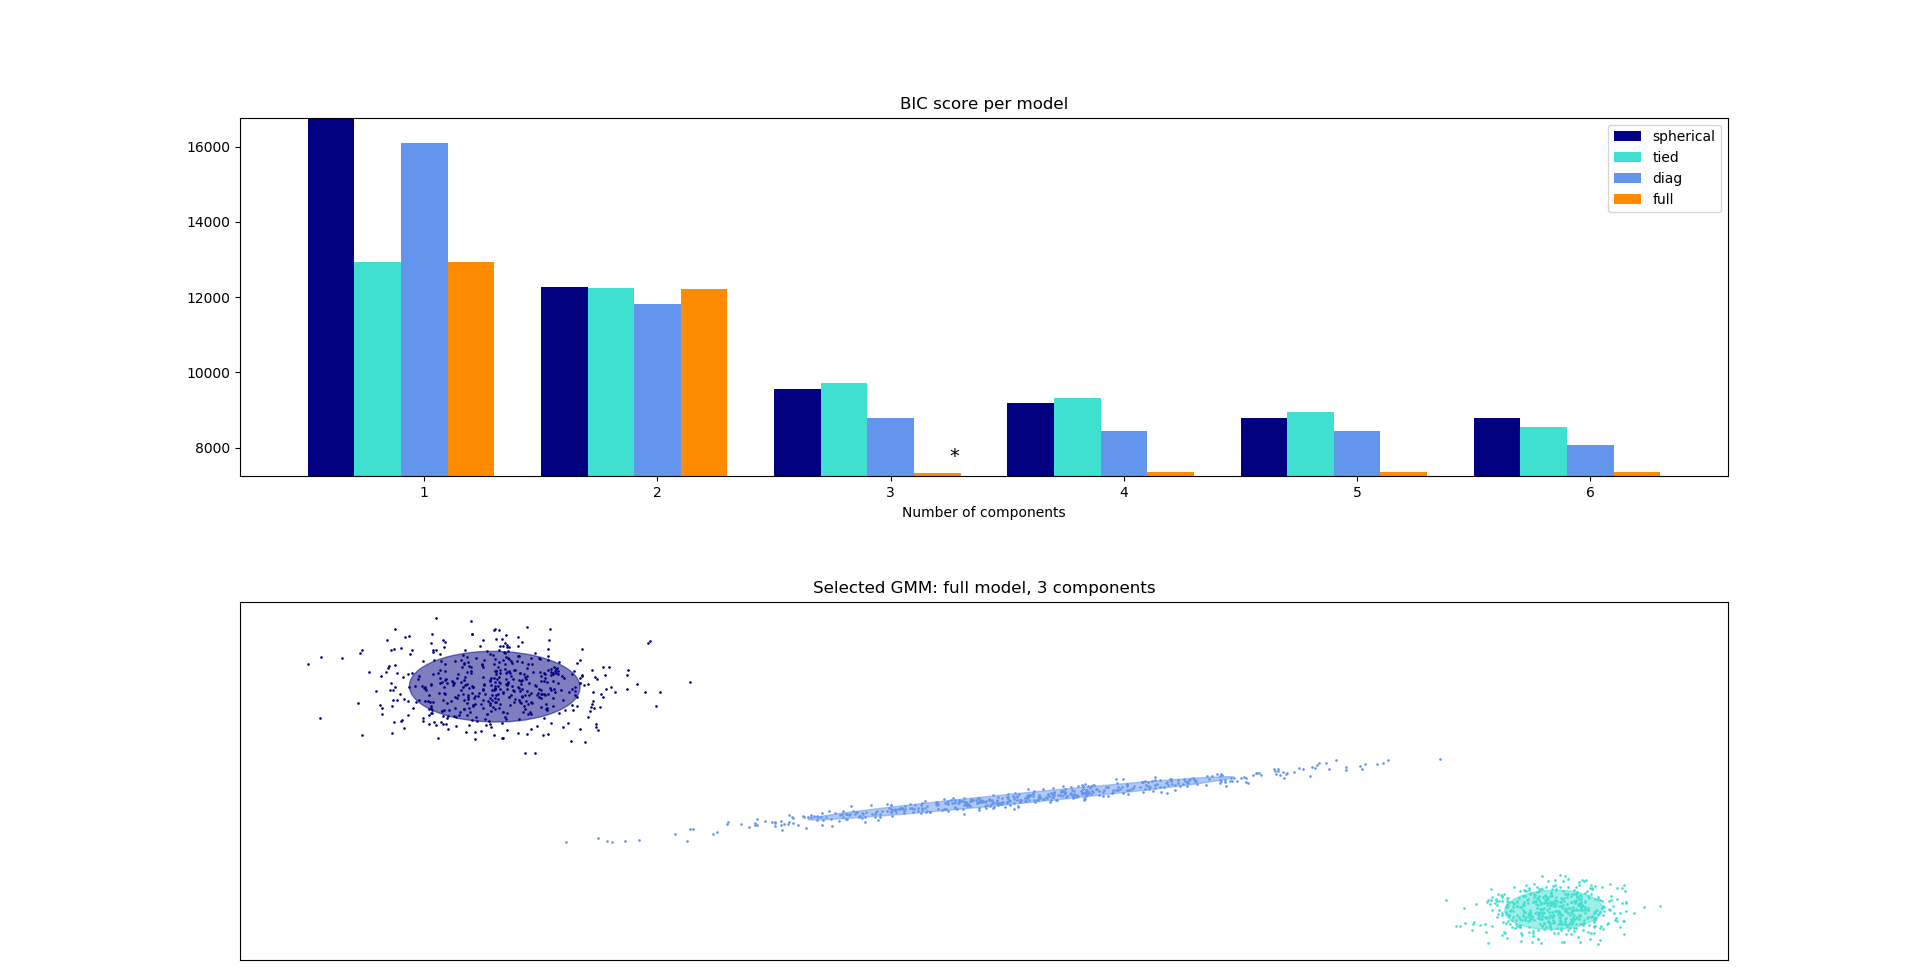
\includegraphics[width=10cm]{problem3/BIC.png}
\caption{BIC score per model}
\label{BIC}
\end{figure}

\subsection{AIC}
Using the sklearn mixture module, we implement a example in Figure \ref{AIC}, first we
 randomly generate datasets based on GMM, in this case, the dataset consists of 3 components, then run the algorithm on the dataset for $k=1\dots 6$, the result is shown in the bar chart, the rectangle with $*$ above it is the best match. It is the model with 4 components and full covariance, which is the true generative model.
\begin{figure}[htbp]
	\centering
	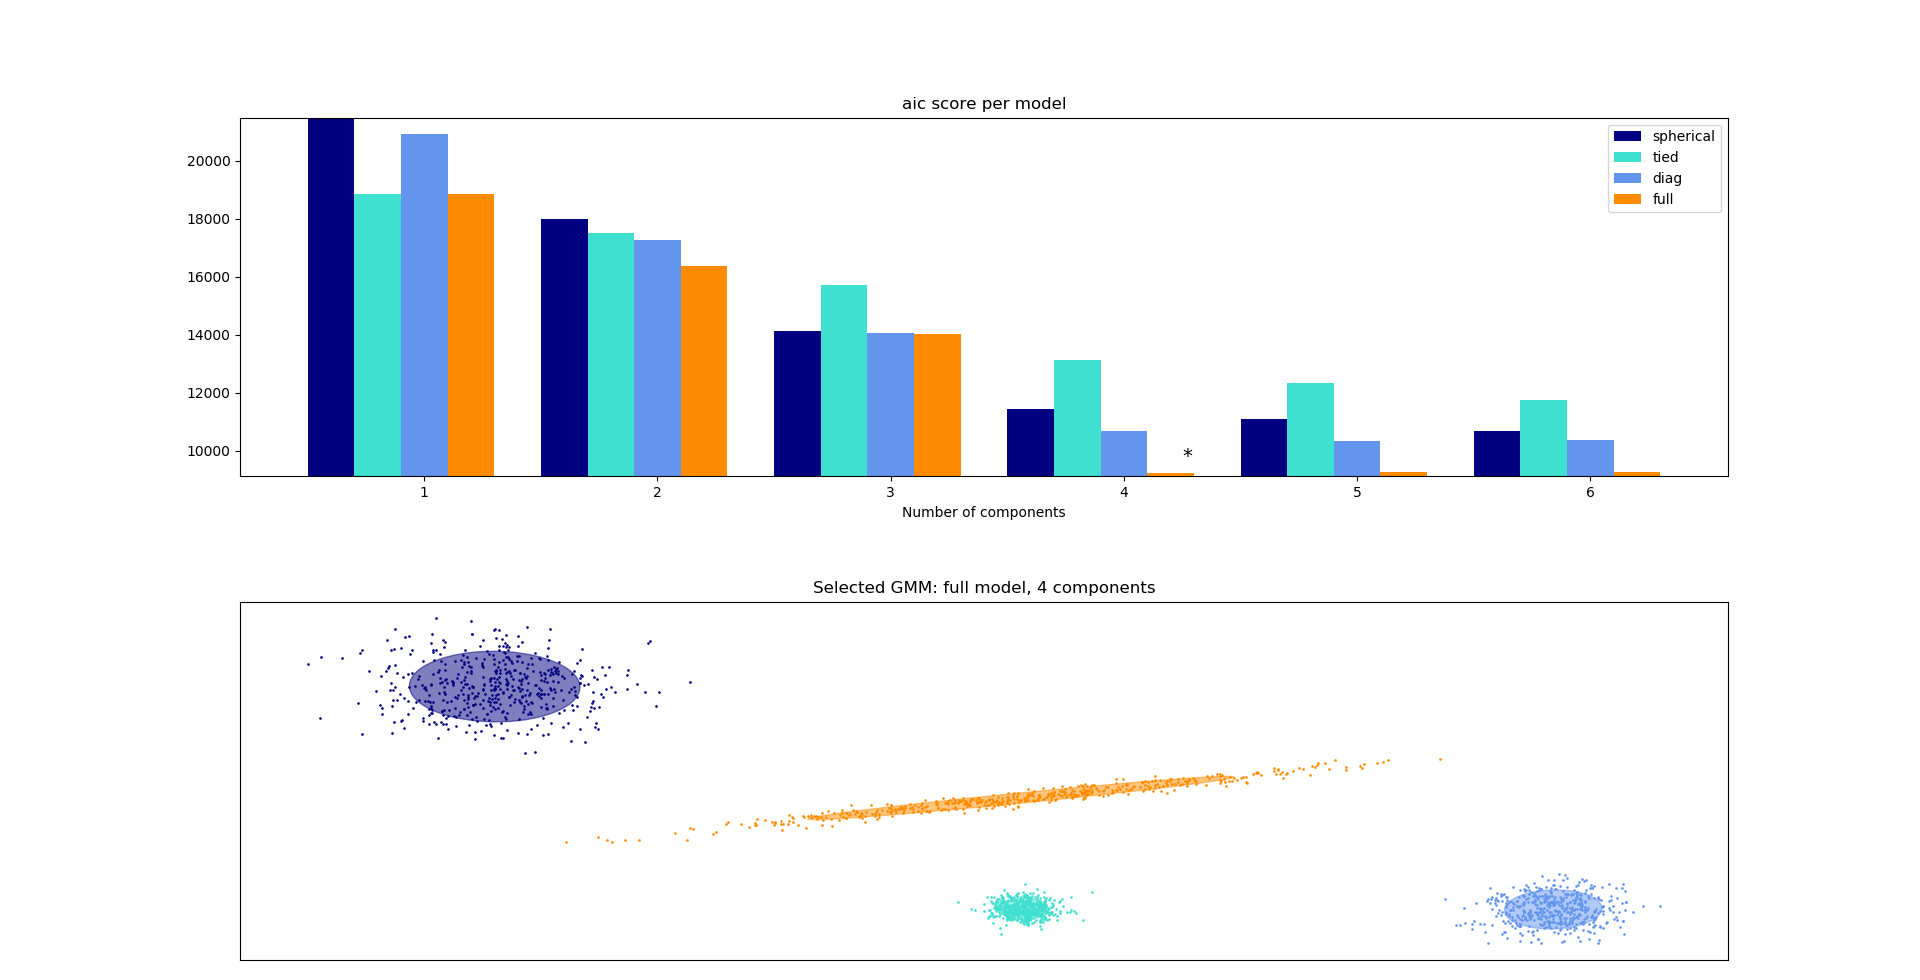
\includegraphics[width=10cm]{problem3/AIC.png}
\caption{AIC score per model}
\label{AIC}
\end{figure}

\subsection{VBEM}
In this part, I implemented the sklearn mixture.BayesianGaussianMixture module. This variational algorithm needs more hyper- parameters than EM algorithm. The most important of these being the concentration parameter weight\_concentration\_prior, which has a strong impact on the effective number of active components obtained. I use the weight parameter ranging from 0.01 to 1000. Another important parameter is weight\_concentration\_prior\_type, which consists of 'dirichlet\_distribution' type and 'dirichlet\_process' type.

Figure \ref{w:1t:dirichlet_distribution},  \ref{w:1000t:dirichlet_distribution}, \ref{w:1t:dirichlet_process}, \ref{w:1000t:dirichlet_process} are some results obtained from changing the two parameters mentioned above, here we can notice that large values for the concentration weight prior lead to more uniform weights when the type of prior is 'dirichlet\_distribution' while this is not necessarily the case for the 'dirichlet\_process' type. Overall this algorithm can select the optimal k automatically. (Pictures of other parameters can be found in the 'picture' folder)
\begin{figure}[htbp]
	\centering
	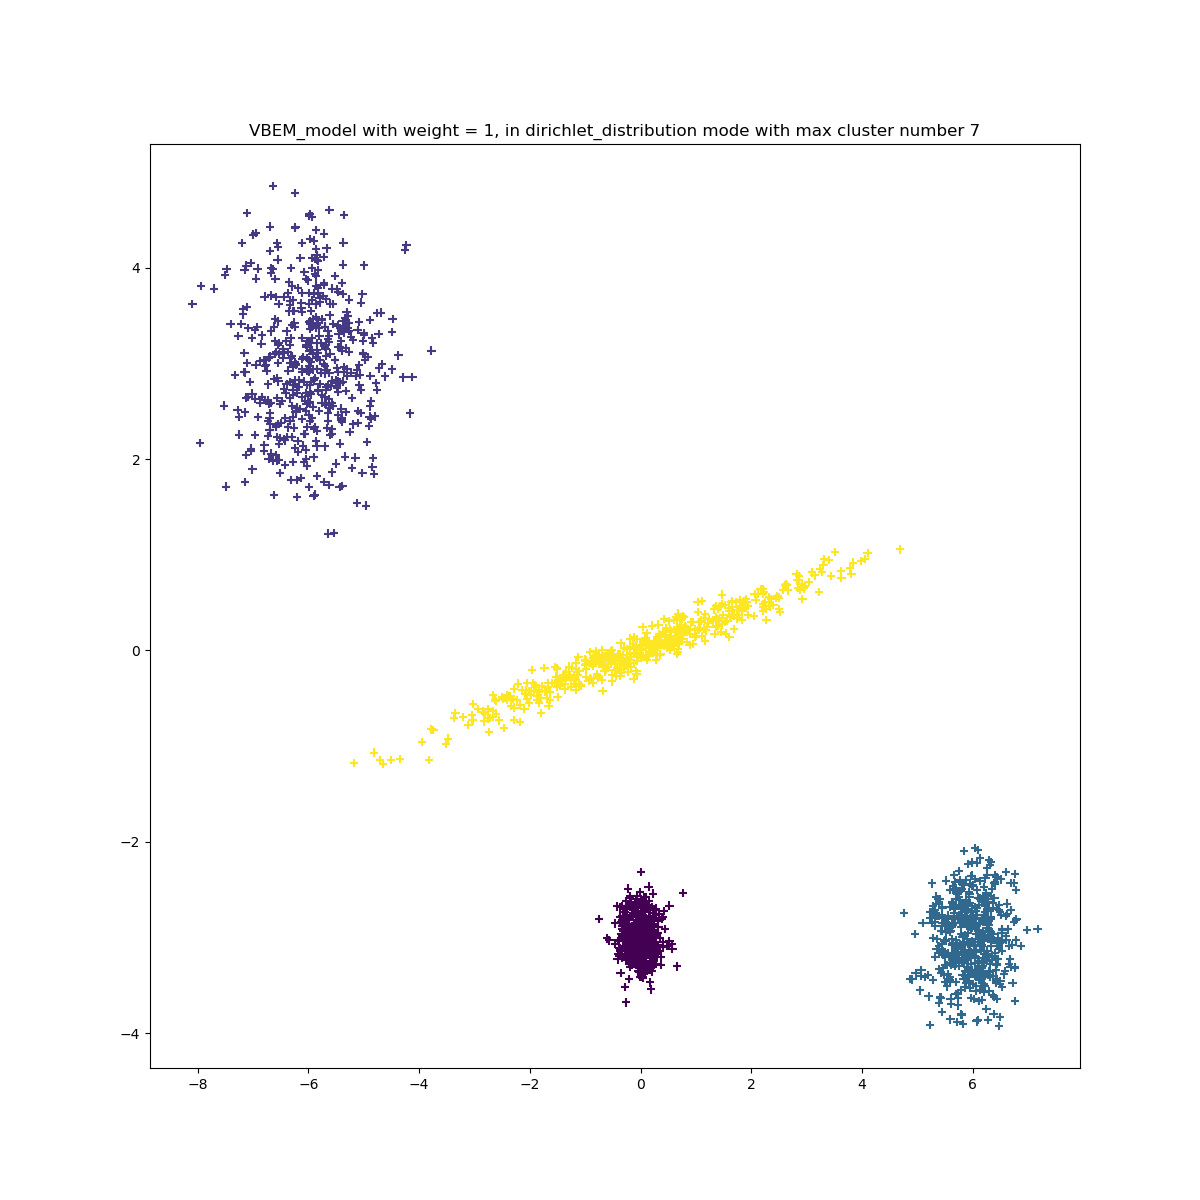
\includegraphics[width=10cm]{problem3/VBEM/w:1t:dirichlet_distribution.png}
\caption{Dirichlet distribution with 1 weight}
\label{w:1t:dirichlet_distribution}
\end{figure}

\begin{figure}[htbp]
	\centering
	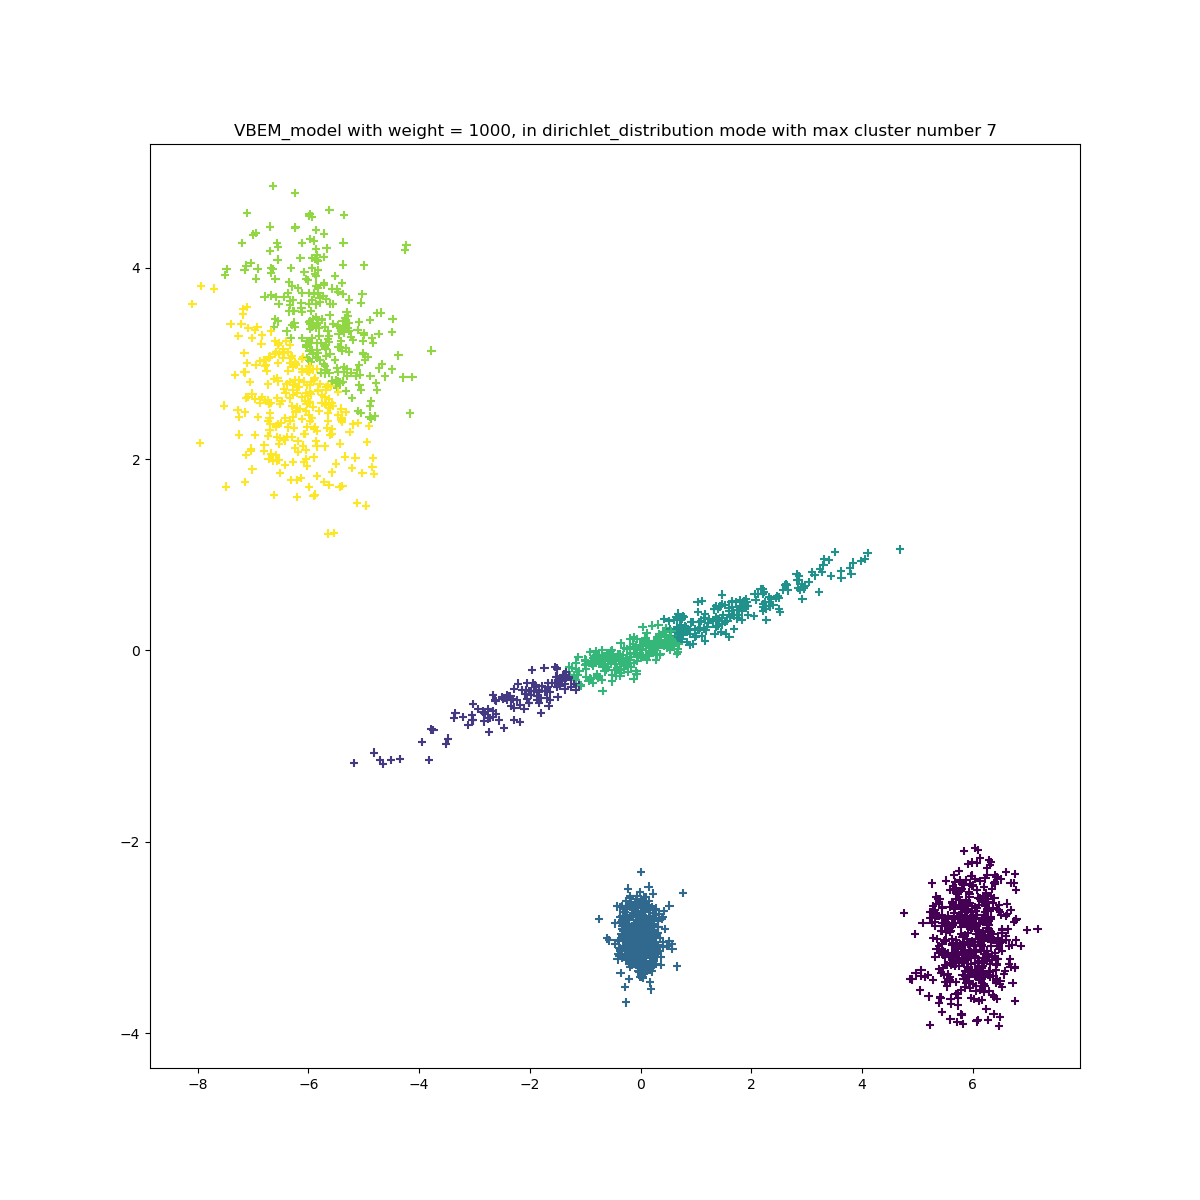
\includegraphics[width=10cm]{problem3/VBEM/w:1000t:dirichlet_distribution.png}
\caption{Dirichlet distribution with 1000 weight}
\label{w:1000t:dirichlet_distribution}
\end{figure}


\begin{figure}[htbp]
	\centering
	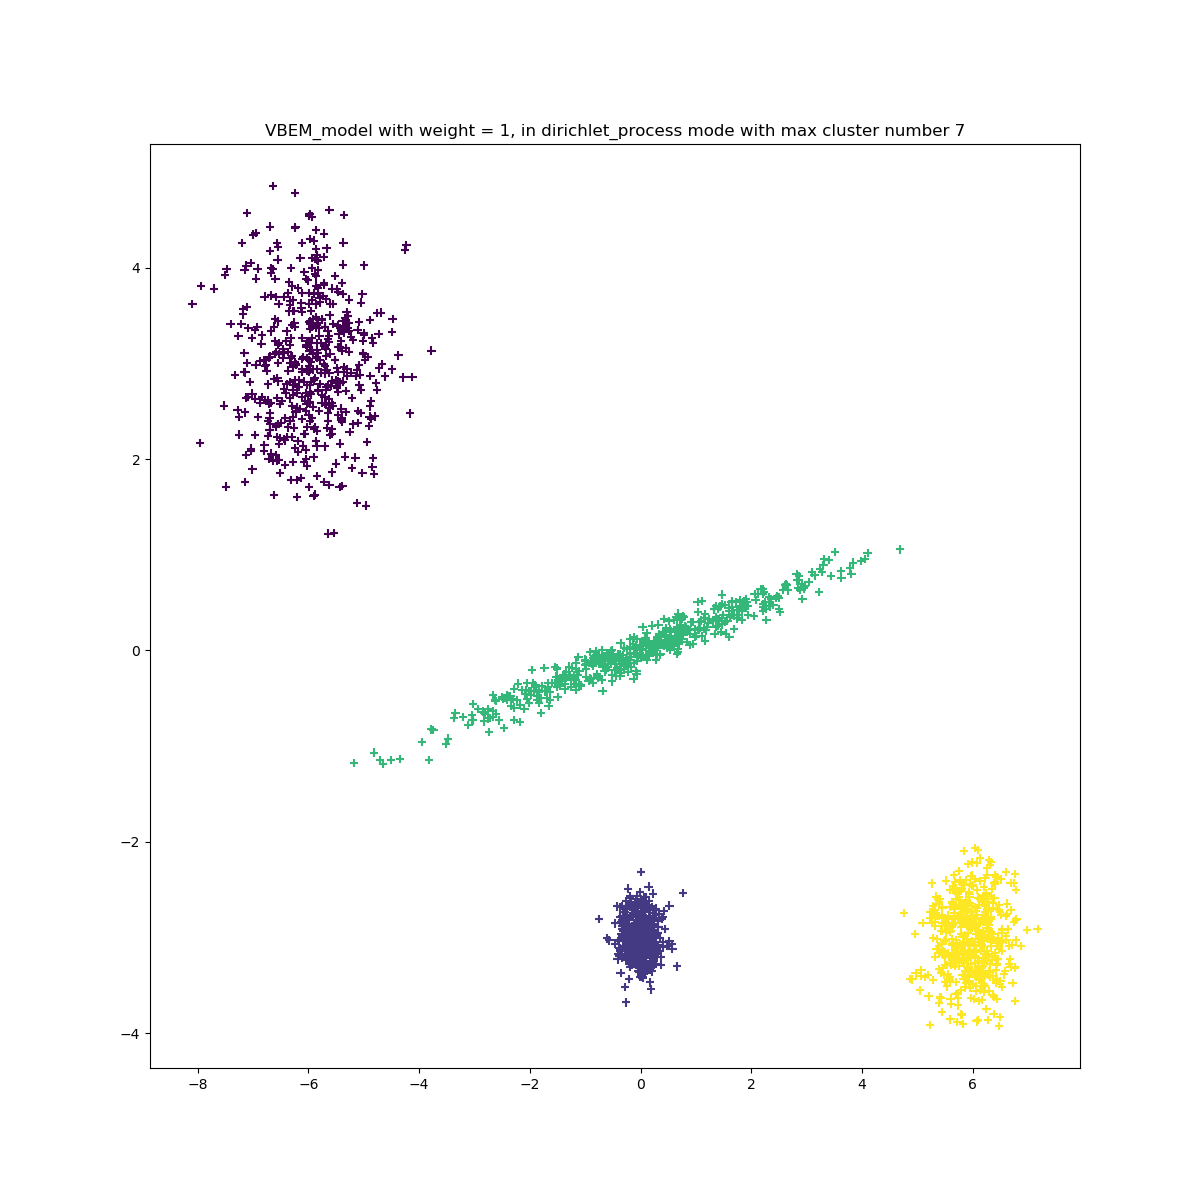
\includegraphics[width=10cm]{problem3/VBEM/w:1t:dirichlet_process.png}
\caption{Dirichlet process with 1 weight}
\label{w:1t:dirichlet_process}
\end{figure}

\begin{figure}[htbp]
	\centering
	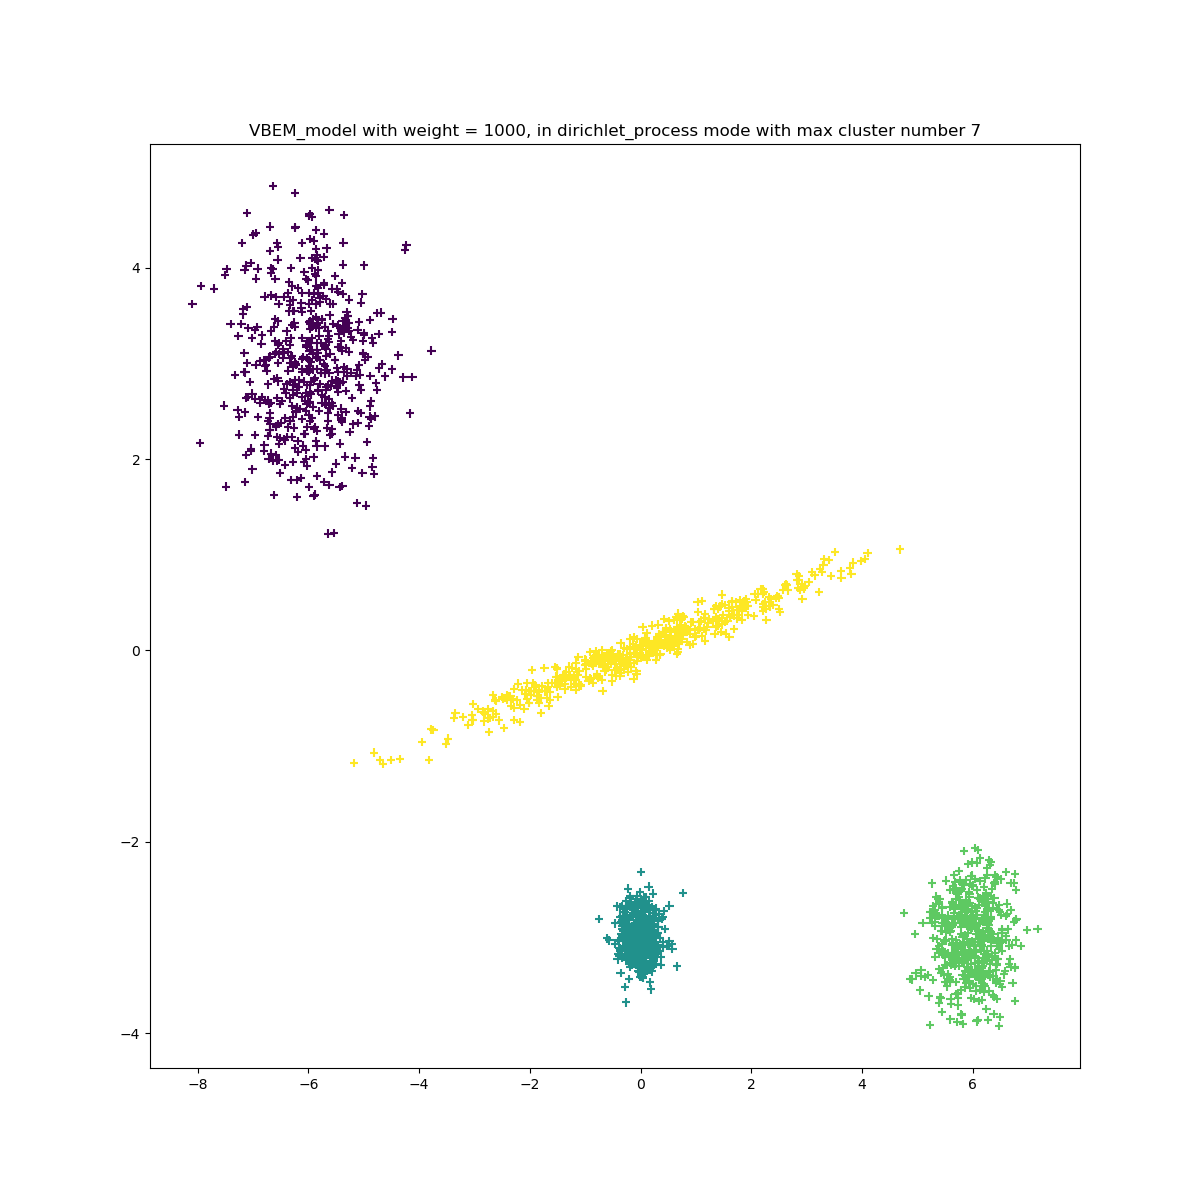
\includegraphics[width=10cm]{problem3/VBEM/w:1000t:dirichlet_process.png}
\caption{Dirichlet process with 1000 weight}
\label{w:1000t:dirichlet_process}
\end{figure}

\hspace{2mm}


%========================================================================
\end{document}
